\documentclass[10pt]{article}
\usepackage[T1]{fontenc}
\usepackage{lmodern}
\usepackage{microtype}
\usepackage[margin=0.86in]{geometry}
\usepackage{amsmath,amssymb}
\usepackage{booktabs,longtable,tabularx,array}
\usepackage{graphicx}
\usepackage{caption}
\usepackage{enumitem}
\usepackage{float}
\usepackage{xcolor}
\usepackage{tikz}
\usetikzlibrary{arrows.meta,positioning}
\usepackage[numbers,sort&compress]{natbib}
\usepackage{hyperref}
\usepackage{fancyhdr}
\usepackage{titlesec}

\definecolor{deepblue}{HTML}{174A7E}
\definecolor{midblue}{HTML}{3B78A8}
\definecolor{pale}{HTML}{EEF5FA}
\definecolor{warm}{HTML}{9B5B2E}
\definecolor{palewarm}{HTML}{FBF1E8}
\definecolor{darkgray}{HTML}{374151}

\hypersetup{colorlinks=true,linkcolor=deepblue,citecolor=deepblue,urlcolor=midblue,pdfauthor={Gang Liu},pdftitle={What Should Count as a Token?}}
\setlength{\parindent}{0pt}
\setlength{\parskip}{0.70em}
\setlist{nosep,leftmargin=1.6em}
\captionsetup{font=small,labelfont=bf}
\titleformat{\section}{\Large\bfseries\color{deepblue}}{\thesection}{0.65em}{}
\titleformat{\subsection}{\large\bfseries\color{darkgray}}{\thesubsection}{0.55em}{}
\titleformat{\subsubsection}{\normalsize\bfseries\color{warm}}{\thesubsubsection}{0.5em}{}
\pagestyle{fancy}
\fancyhf{}
\lhead{What Should Count as a Token?}
\rhead{Working Draft}
\cfoot{\thepage}
\setlength{\headheight}{14pt}

\newcolumntype{Y}{>{\raggedright\arraybackslash}X}
\newcolumntype{L}[1]{>{\raggedright\arraybackslash}p{#1}}
\newcommand{\term}[1]{\textbf{#1}}
\newcommand{\status}[1]{\textbf{#1}}
\newcommand{\topic}[1]{\par\smallskip\noindent\textbf{#1.}\ }
\newcommand{\draftsuggestion}[1]{\begin{center}\fcolorbox{warm}{palewarm}{\parbox{0.92\linewidth}{\textbf{Draft suggestion:} #1}}\end{center}}
\newcommand{\principle}[1]{\begin{center}\fcolorbox{deepblue}{pale}{\parbox{0.92\linewidth}{#1}}\end{center}}
\newcommand{\observation}[1]{\begin{center}\fcolorbox{warm}{palewarm}{\parbox{0.92\linewidth}{#1}}\end{center}}


\title{What Should Count as a Token?\\
\large A Comprehensive Study of Data Representation for Foundation Models}
\author{TODO}
% \date{September 2026}
\date{}

\begin{document}
\maketitle

\begin{abstract}

\draftsuggestion{
Foundation models operate on finite collections of addressable units, yet the choice of these units often receives less study than the architecture that processes them. Tokenization determines unit boundaries, representation scale, retained information, explicit relations, and computational allocation. These choices are especially important in science, where measurement units may differ from the structural or functional units required by a task. We define a tokenizer as a three-module system that constructs reusable parameters, maps an input to a token representation, and maps that representation to a reconstruction. This definition covers algorithmic, neural, and hybrid tokenizers while separating token formation from the downstream foundation model.
}


\draftsuggestion{We study how these methods define tokens for different AI modalities and scientific domain objects, identifying the component tokenizers used to represent individual data sources or objects. 
We also study system-level tokenization for complex settings that combine multiple modalities, domain objects, spatial or temporal scales, and coupled observations and actions. }

\draftsuggestion{Across these levels, we examine the trade-offs among coverage, compression, reconstruction, task information, scientific constraints, and model compatibility. We conclude with design principles, evaluation protocols, and a research agenda for adaptive, multiscale, and reusable tokenizers that support future foundation models in prediction, generation, and interaction.}



\draftsuggestion{\textbf{Note: Please add your references in a separate bib file in the bib folder. Please reuse the citation if warnings are raised; don't worry about the same paper with different cite-ids }}

\end{abstract}

\tableofcontents
\newpage

\section{Introduction}
\label{sec:introduction}

\draftsuggestion{Extend the related-work coverage by searching for unit formation under segmentation, compression, patching, pooling, quantization, motif discovery, grammar induction, discretization, and state abstraction. Prioritize papers that introduce or directly evaluate tokenization. Retain reuse-only systems when they have broad impact, document a major public model, or supply a comparison that is missing from the review.}

\subsection{Motivation, Scope, and Contributions}

\draftsuggestion{State the intended readers, the inclusion rule, and the three contributions in terms that can be checked against the catalog. Keep examples representative rather than exhaustive. Present AI modality and domain object as two views of component tokenizers, then present complex systems as the composition of those components across modalities, objects, scales, or time.}

% Foundation models convert observed data into finite collections of model inputs. Language systems may use words, subwords, characters, or bytes. Vision systems may use pixels, patches, regions, or latent codes. Scientific models may use atoms, molecular fragments, residues, gene identifiers, mesh cells, or spectral peaks. The selected units determine what a model can address, compare, mask, predict, and allocate computation to.

% The literature does not use one name for this design choice. Relevant methods appear under segmentation, compression, patching, pooling, clustering, vector quantization, motif discovery, grammar induction, discretization, and state abstraction. We include a method when it constructs or selects finite addressable units for model input, output, intermediate computation, or reconstruction. This rule includes methods that do not use the word \emph{tokenization} but satisfy the definition in Section~\ref{sec:tokenizer-definition}.

% The review gives priority to papers that introduce a tokenizer, define one of its modules, or evaluate tokenization directly. We retain a system that only reuses an existing tokenizer when it provides an influential reference point, documents a major public model, or isolates a design choice that other retained papers do not test. This rule keeps the review focused while preserving evidence needed to compare tokenizers in practice.

% The scope covers symbolic sequences, images, video, audio, three dimensional geometry, graphs, tables, time series, fields, and spectra. Scientific sections study biological, chemical, physical, Earth, clinical, and embodied objects. A separate section examines systems that join modalities, objects, scales, or temporal states. The main object of analysis is a \term{tokenizer system} with training, encoding, and decoding modules. Section~\ref{sec:tokenizer-definition} states when a paper defines the full system and when it defines only one component.

% The paper makes three contributions. First, it gives a common mathematical definition for fixed alphabets, learned vocabularies, continuous units, and discrete neural codebooks. Second, it separates construction method, AI modality, domain object, and complex-system composition. Third, it defines evaluation controls that distinguish information retention, scientific validity, downstream utility, and compute cost.

\subsection{From Compression to Intelligence}

\draftsuggestion{Trace the technical line from coding and dictionary compression to subword learning, vector quantization, fixed patches, and learned unit selection. Emphasize which ideas changed tokenizer training, encoding, or decoding. Avoid presenting the history as a sequence of foundation-model architectures.}

% Tokenization links coding, compression, and statistical prediction. Information theory formalized the relation between symbol probabilities and code length \citep{shannon1948}. Later text systems learned reusable variable-length units from a corpus. Byte pair encoding (BPE) was adapted to open-vocabulary neural machine translation \citep{sennrich2016}. This example shows that the vocabulary and the segmentation rule are separate parts of a tokenizer.

% Vision and audio systems developed related choices. Vision Transformers expose fixed image patches as model units \citep{dosovitskiy2021vit}, while vector-quantized models learn discrete codes from continuous signals \citep{oord2017vqvae}. These examples separate three operations: forming boundaries, computing token values, and optionally mapping values to a finite codebook.

% Relational and scientific data study structures that a flat sequence does not represent directly. Graph tokenizers may use nodes, walks, or subgraphs. Molecular tokenizers may use string symbols, atoms, fragments, or grammar rules. Protein and cellular models may use residues, local structures, genes, or learned states. Across these cases, a token has limited meaning unless the representation also contains order, adjacency, geometry, or another relation.

% These systems share a common design pattern. A method chooses a base representation, forms units at one or more scales, stores relations, and defines what can be recovered. Its modules may be algorithmic, neural, or hybrid. Section~\ref{sec:tokenizer-systems} defines this pattern. Sections~\ref{sec:ai} and~\ref{sec:science} compare component tokenizers by AI modality and domain object. Section~\ref{sec:joint-systems} studies their composition in complex systems, and Section~\ref{sec:principles} states how competing choices can be tested.

\subsection{Observations and Insights}

\draftsuggestion{\textbf{Tokenizer systems are often compared only through their output units.} Test whether reported conclusions change after separating tokenizer training, encoding, and decoding. Useful cases include subword vocabularies with different segmentation rules, visual codebooks with different decoders, and molecular vocabularies with incomplete inverse mappings. Keep this observation provisional until each case has direct evidence.}

\draftsuggestion{\textbf{Scientific token identity often depends on relations and scale.} Compare atoms with motifs, residues with structure units, genes with cell states, and grid cells with adaptive regions. Record when geometry, symmetry, experimental condition, or task changes the useful unit. Include cases where fixed small units remain the stronger choice.}

\draftsuggestion{\textbf{Compression, reconstruction, and scientific utility can disagree.} Look for tokenizers that reduce sequence length or reconstruction error while losing rare events, valid composition, intervention response, or transfer information. Compare the tokenizer training objective with every later evaluation target before making a general claim.}

\begin{figure}[t]
    \centering
    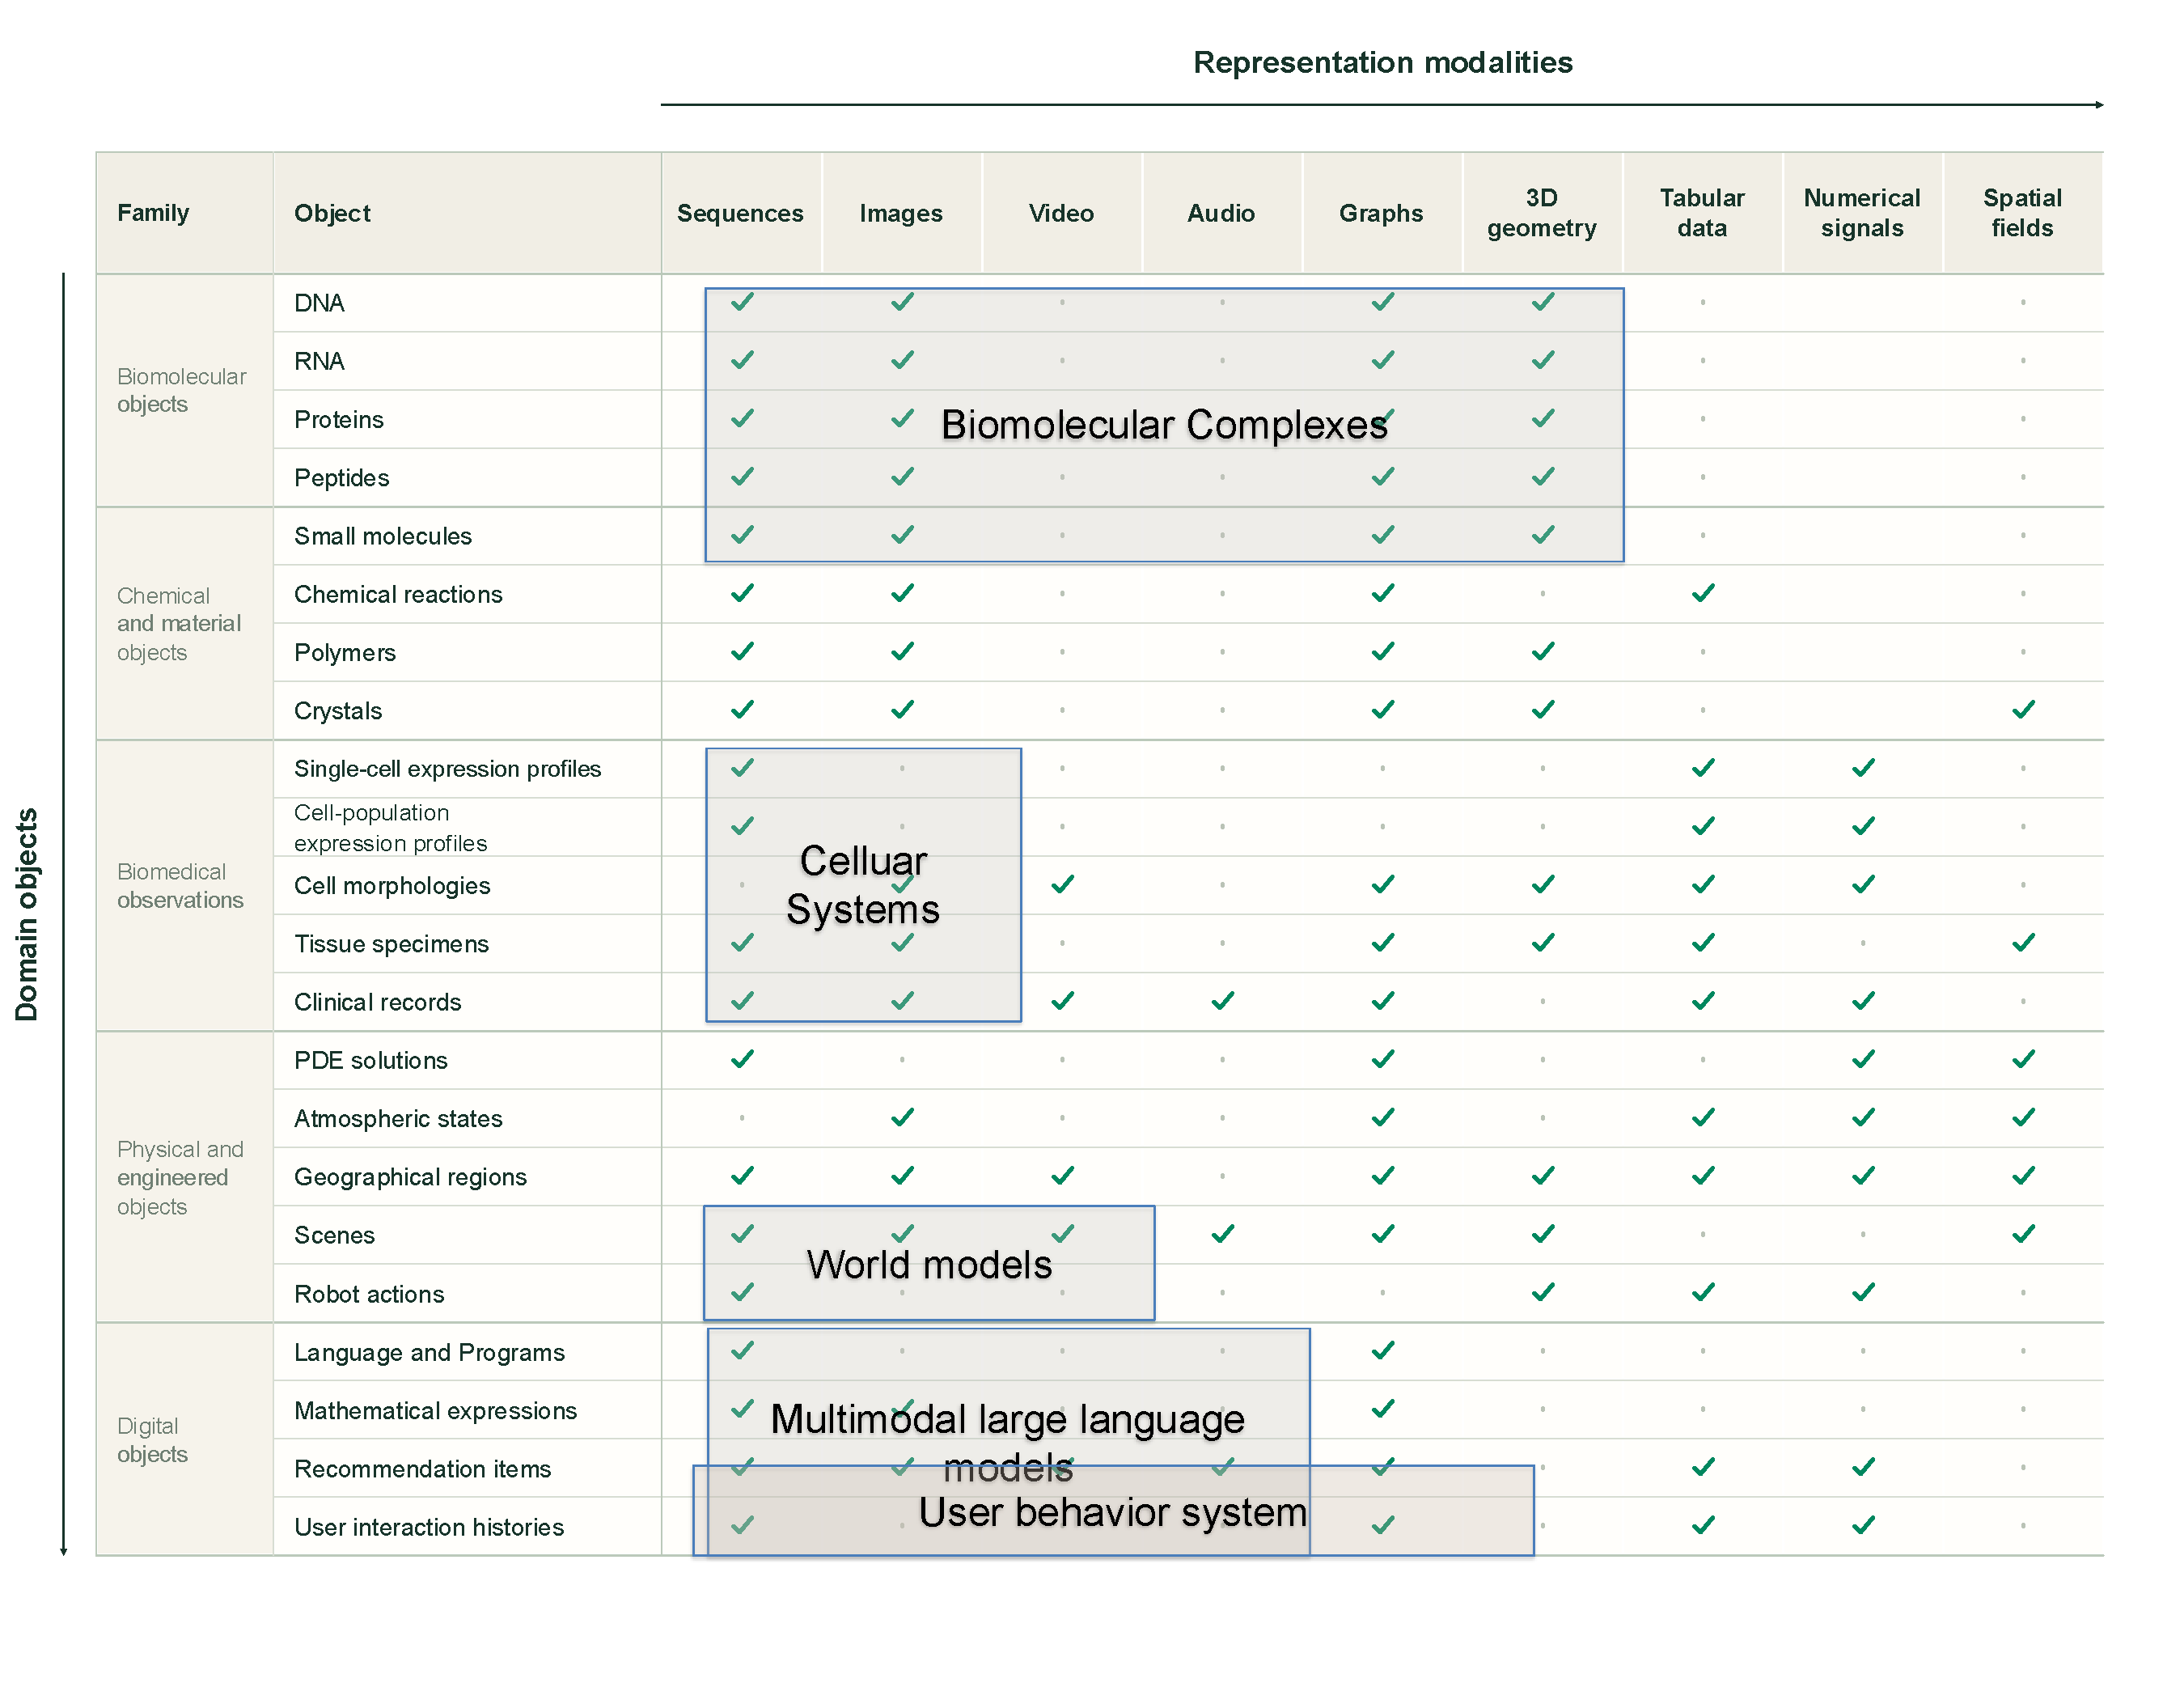
\includegraphics[width=\linewidth]{figures/overview.pdf}
    \caption{Overview of the work: We organize the review into two major dimensions (representations and objects). (The current tick is tentative; feel free to let me know your suggestion and to remove or add new ticks based on your survey.)}
    \label{fig:overview}
\end{figure}
\section{Tokenizer Systems: Definition and Method Taxonomy}
\label{sec:tokenizer-systems}

\draftsuggestion{Use the three-module definition as the common comparison frame for every method family. Classify only the operations that determine token units, assignments, or reconstruction. Keep embedding layers, foundation-model backbones, and task heads outside the tokenizer unless they change one of these operations.}

% This section defines the object studied throughout the paper. The definition separates token formation from the foundation model that later processes the tokens. It also applies to symbolic vocabularies, continuous latent units, discrete neural codes, and structured scientific objects.

\subsection{A Tokenizer as a Three-Module System}
\label{sec:tokenizer-definition}

\draftsuggestion{Keep the definition independent of modality and downstream architecture. Explain the roles of \texttt{train}, \texttt{encode}, and \texttt{decode} through BPE, VQ-VAE, and fixed image patches. State the reconstruction and equivalence rule for lossy or structured data, then use the definition to separate full tokenizers from methods that specify only one module.}

Let $\mathcal{X}$ denote an input space and $\mathcal{Z}$ a token space. We define a tokenizer system as
\begin{equation}
\mathcal{T}
=\bigl(\operatorname{train},\operatorname{encode},\operatorname{decode}\bigr),
\label{eq:tokenizer-triple}
\end{equation}
with operations
\begin{equation}
\theta=\operatorname{train}(\mathcal{D}),
\qquad
Z=\operatorname{encode}_{\theta}(x),
\qquad
\widehat{x}=\operatorname{decode}_{\theta}(Z).
\label{eq:tokenizer-system}
\end{equation}
Here, $\mathcal{D}$ is the data used to construct or fit the tokenizer, $x\in\mathcal{X}$ is an input, $Z\in\mathcal{Z}$ is its token representation, and $\widehat{x}\in\mathcal{X}$ is the reconstructed input. We use $\theta$ for all reusable quantities returned by training. These quantities may include a vocabulary, merge table, or codebook. They may also include deterministic rules or neural parameters. A predefined tokenizer is the special case $\operatorname{train}(\mathcal{D})=\theta_0$ for every $\mathcal{D}$.
For a structured input, the encoded representation can be written as
\begin{equation}
Z=\bigl((z_i)_{i=1}^{n},R\bigr),
% \qquad n<\infty,
\label{eq:structured-tokens}
\end{equation}
where $z_i$ is one token and $R$ records any relations required to interpret the token collection. Sequence order can define $R$ implicitly. Graph edges, spatial coordinates, or hierarchical links may define it explicitly. A unit qualifies as a token when a later model can process it separately for masking, prediction, or routing. The decoder recovers what information the tokenizer preserves. Exact recovery requires
\begin{equation}
\operatorname{decode}_{\theta}
\bigl(\operatorname{encode}_{\theta}(x)\bigr)=x.
\label{eq:exact-roundtrip}
\end{equation}
Some domains have several records for the same object. In such cases, recovery may be defined up to a stated equivalence, such as graph isomorphism, geometric symmetry, or text normalization. Continuous data usually require an approximation for reconstruction rather than equality. Therefore, the reconstruction target and its comparison rule are part of the tokenizer definition.

We categorize tokenizers into three classes based on how their training algorithms are defined: (1) algorithmic tokenizers, (2) neural tokenizers, and (3) hybrid tokenizers. Algorithmic tokenizers use non-neural training algorithms, which can be either predefined or data-driven, whereas neural tokenizers rely on generative models and quantization techniques.

Byte pair encoding (BPE) is an example of an algorithmic tokenizer. Its training function constructs a vocabulary and an ordered merge table from corpus statistics. The encoding function applies the learned merges to a new sequence, while the decoding function concatenates the resulting symbols.

Another example of an algorithmic tokenizer is image patching, as used in the Vision Transformer (ViT)~\citep{dosovitskiy2021vit}. In this predefined tokenizer, $\theta_0$ specifies the patch size and ordering. In contrast, vector-quantized variational autoencoders (VQ-VAEs) are examples of neural tokenizers~\citep{oord2017vqvae} and have been adapted to continuous and non-discrete data. In the following subsections, we define these three classes in detail.


% Equations~\eqref{eq:tokenizer-triple}--\eqref{eq:vq-example} also separate a full tokenizer system from one of its components. A vocabulary-learning algorithm alone specifies part of \texttt{train}; a pooling rule alone specifies part of \texttt{encode}; and a generator is a tokenizer decoder only when it reconstructs the input object. 

\subsection{Algorithmic Tokenizers}
\label{sec:algorithmic-tokenizers}

BPE-like

\draftsuggestion{Develop this subsection around the three sources of unit formation rather than a long list of algorithms. For each family, compare what \texttt{train} estimates, how \texttt{encode} resolves competing segmentations, what \texttt{decode} recovers, and which choices introduce randomness. Select a small number of examples from text, signals, graphs, and scientific structures.}

% Algorithmic tokenizers determine tokens without a trained neural network. We separate them by the source of the unit-forming rule. Predefined-unit methods specify units directly, as with amino acid residues and fixed image patches \citep{rives2021esm,dosovitskiy2021vit}. Expert-defined composition constructs units with designed rules, as in the temporal aggregation and symbolic discretization used by Symbolic Aggregate approXimation \citep{lin2003sax}. Data-learned composition estimates non-neural rules from observations, as in BPE \citep{sennrich2016}.

% This division concerns token formation rather than the model that consumes the tokens. Data fitting does not by itself make a tokenizer neural. Pair counts, likelihood objectives, clustering, grammar induction, and numerical optimization can all produce learned vocabularies without a neural network. Conversely, a later Transformer or diffusion model does not change the tokenizer class when it only processes previously formed units.

\subsection{Neural and Hybrid Tokenizers}

\draftsuggestion{Ask section authors to identify the last operation that changes token identity or membership. Use that boundary to distinguish the tokenizer from embedding layers, backbones, task heads, and generators. Compare neural systems by their learned token operation and compare hybrid systems by how the algorithmic and neural stages are composed.}


A vector-quantized variational autoencoder (VQ-VAE) gives a neural example~\citep{oord2017vqvae}. The training function jointly learns a neural network encoder $f_{\phi}$, a codebook $C=\{c_j\}_{j=1}^{K}$, and a neural network decoder $g_{\psi}$. For each local feature, the encoding function assigns
\begin{equation}
k_i=\arg\min_{1\leq j\leq K}
\left\lVert f_{\phi}(x)_i-c_j\right\rVert_2,
\qquad
\widehat{x}=g_{\psi}(c_{k_1},\ldots,c_{k_n}).
\label{eq:vq-example}
\end{equation}
The tokens are the code indices $(k_i)_{i=1}^{n}$, and decoding is generally approximate. The codebook is part of $\theta$.

% Neural tokenizers require trained neural parameters to determine the final addressable units. Standard tensor operations inside such a system, including nearest-code lookup, do not by themselves create a separate algorithmic tokenizer. We group neural systems first by token form and then by unit layout. Quantized latent tokenizers map neural features to discrete codes, as in VQ-VAE \citep{oord2017vqvae}. Among continuous systems, selected or composed tokenizers learn input-dependent unit membership, as in TokenLearner \citep{ryoo2021tokenlearner}. Fixed-layout continuous tokenizers retain predefined positions while learning their latent values. This decision rule assigns a discrete system to the quantized family even when its encoder also performs selection or composition.

% Hybrid tokenizers combine neural token formation with a separate algorithmic rule of the type defined in Section~\ref{sec:algorithmic-tokenizers}. Both parts determine the final addressable units. We distinguish three system structures. Joint systems couple the two parts in one unit-formation rule. Sequential systems pass the units from one tokenizer stage into another. Parallel-stream systems retain separate token sequences before the model combines them. Byte Latent Transformer provides a representative sequential system in which learned patches are formed over bytes \citep{pagnoni2025blt}.

% The classification must follow the token-forming path. A neural encoder followed by quantization defines a neural tokenizer even when its decoder is a diffusion model. A non-neural composition rule remains algorithmic when a later neural model only processes the resulting units. The tokenizer and the full foundation-model system therefore require separate descriptions.

% \section{Review Scope and Literature Coding}
\label{sec:review-protocol}

\draftsuggestion{Document how the authors search for papers that may not use the word tokenization. Keep the protocol broad enough for a field study and precise enough that a later revision can report a reproducible screening flow. The companion catalog should remain the source of record for inclusion decisions and tokenizer-system extraction.}

\subsection{Search Scope and Inclusion Rule}

\draftsuggestion{State the search cutoff, source types, query families, and inclusion rule. Explain how the search finds tokenizer work published under segmentation, quantization, pooling, discretization, grammar induction, or state abstraction. Report the screening flow only after a second author checks exclusions and duplicate records.}

The search covers work published or publicly posted through September 6, 2026. It begins with compression, segmentation, clustering, quantization, parsing, and scientific representation methods from the twentieth century. Coverage becomes denser after 2016, when subword tokenization and Transformer models made token units a central system choice. The search uses publisher pages, conference proceedings, archival repositories, citation trails from review papers, official technical reports, public model cards, and released tokenizer files.

A record enters the main catalog when it performs at least one of three functions. It forms finite units from a finer representation, maps observations to a finite or addressable latent set, or changes the units used to allocate model computation. This rule includes fixed patches, learned pooling, vector quantization, graph motifs, spectral peaks, ranked genes, and mesh nodes. A record is contextual when it supplies relevant foundation-model information but neither defines nor tests token formation.

Search terms combine each data type in Sections~\ref{sec:ai} and \ref{sec:science} with method terms such as \emph{tokenization}, \emph{segmentation}, \emph{discretization}, \emph{vector quantization}, \emph{codebook}, \emph{patching}, \emph{pooling}, \emph{motif vocabulary}, \emph{grammar induction}, \emph{structure alphabet}, \emph{state abstraction}, and \emph{adaptive mesh}. The authors should preserve query dates and sources in the supplement before submission.

\subsection{Tokenizer-System Extraction}

\draftsuggestion{Extract \texttt{train}, \texttt{encode}, and \texttt{decode} from the primary paper, released code, or official model files. Record which operation determines token identity, which output can be decoded, and which later neural layers belong to the foundation model rather than the tokenizer.}

For every core paper, the review extracts bibliographic identity, data object, input space, token space, relation structure, and the three modules from Section~\ref{sec:tokenizer-definition}. Training fields record data, objective, fitted components, randomness, constraints, and cost. Encoding fields record boundary formation, assignment, output form, relations, and inference randomness. Decoding fields record the target space, exactness, canonicalization, reconstruction method, validity checks, and missing information.

The classification separates a tokenizer from the model that consumes its output. A fixed image partition belongs to the tokenizer because it determines patch units. A learned projection belongs to token formation only if the study defines token identity through the projected vectors. Later self-attention layers belong to the backbone unless they merge, prune, route, or reform addressable units. A molecular generator counts as tokenizer decoding only when it maps tokens to the declared molecular reconstruction target.

Each field receives one of four evidence labels: stated by the source, derived from equations or released code, inferred by the reviewers, or unreported. Inference should remain short and testable. The review must not infer exact reversibility from discrete identifiers or infer stochastic behavior from the presence of a neural network.

\subsection{Taxonomy Assignment and Evidence Limits}

\draftsuggestion{Assign record type, implementation basis, method family, module coverage, AI modality, domain object, and complex-system setting as separate dimensions. Require direct evidence before assigning a complex-system setting; several modality labels alone do not show that the tokenizer combines component token streams.}

The review records distinct questions in separate dimensions. It distinguishes the contribution of a source from the implementation that forms its tokens. Method family refines the implementation basis, while module coverage records whether the source specifies training, encoding, and decoding. AI modality names the representation form, domain object names what is represented, and complex-system setting records how component tokenizers are combined. This structure prevents a paper's scientific topic or model architecture from determining its tokenizer class.

For example, a protein paper may have sequence and geometry modalities and protein as its domain object. SaProt uses composed algorithmic and neural token streams, while a later protein language model remains outside token formation. A theoretical paper receives a record type but no implementation basis.

The paper catalog is intentionally broader than the set used for direct performance comparison. Direct comparison requires compatible data splits, base units, backbone capacity, optimization budget, token budget, and evaluation target. Papers with incompatible settings remain part of the historical and design record, but their reported numbers should not be ranked in one table.

No literature search can establish a literal set of all related papers because method names and indexing differ across fields. The authors should call the catalog \emph{comprehensive within the stated scope}, report the cutoff date, and keep a public route for corrections. This wording makes the search boundary clear while allowing the catalog to grow.

The current catalog, system table, and model profiles are working evidence rather than final study results. Descriptive counts should enter the manuscript only after duplicate removal, a second review of the main systems, and reconciliation between the Markdown and spreadsheet records. A checkpoint that reuses an existing tokenizer should remain a model profile rather than being counted as a new tokenizer method.

\draftsuggestion{Report the final search dates, screening flow, inter-reviewer agreement, and descriptive counts in this section or an appendix. Keep model-card evidence separate from peer-reviewed method evidence. State all missing implementation details as unreported rather than inferring them from the foundation-model architecture.}

\section{Data Representation and Tokenization across AI Modalities}
\label{sec:ai}

\draftsuggestion{Write this section for machine learning researchers and organize it by representation form. Use general AI tasks and models to compare token units, relations, training objectives, decoding targets, token rates, and computational cost. Mention scientific examples such as SMILES strings, protein sequences, molecular graphs, or physical trajectories only briefly, then refer readers to Section~\ref{sec:science} for their object-specific meaning and tests. This section should explain transferable tokenization methods rather than repeat the scientific-object review.}

% An AI modality specifies how information is represented rather than what the represented entity is. The same scientific object may therefore appear in several subsections. A protein, for example, can be represented as a sequence, graph, three dimensional structure, or time series. This organization supports method transfer while keeping scientific meaning for Section~\ref{sec:science}. We discuss spatial fields and spectra with their primary scientific objects because the current tokenizer literature ties their unit definitions closely to coordinates, measurements, and validation rules.

\subsection{Sequences}

[zhenyu]

\draftsuggestion{Representative work: \citet{sennrich2016}. Treat a sequence as an ordered representation and compare characters, bytes, subwords, words, and syntax-aware units. Use text and code as the main AI cases. Discuss coverage, sequence length, reversibility, multilingual behavior, and syntactic structure. Mention SMILES, nucleic-acid sequences, and protein sequences only as short transfer examples, then refer readers to Section~\ref{sec:science}.}

% Text can be represented by words, characters, bytes, or subwords. Word vocabularies are readable but have limited coverage. Character and byte systems cover any input but produce longer sequences. Subword methods learn intermediate units from corpus statistics and balance coverage against sequence length \citep{sennrich2016}.

% Code adds formal syntax and long-range references. A token may correspond to a keyword, part of an identifier, whitespace, or punctuation. Frequency-based segmentation can divide the same identifier differently across repositories. Parser-based units preserve grammar roles but depend on valid syntax and may remove surface form.

% Symbolic sequences use a finite alphabet whose symbols may represent bases, amino acids, events, or other ordered observations. Their units can be predefined or composed from repeated patterns. Scientific meaning and evaluation remain tied to the domain objects discussed in Section~\ref{sec:science}.

\subsection{Images}

\draftsuggestion{Representative work: \citet{dosovitskiy2021vit} and \citet{oord2017vqvae}. Compare pixels, fixed patches, regions, object-level units, and latent visual codes for recognition and generation. Separate token boundaries from token values and compare reconstruction, token rate, spatial resolution, and compatibility with vision backbones. Treat scientific grids as images only when their row-and-column layout defines the model input; discuss their scientific meaning in Section~\ref{sec:science}.}

% Images can be divided into pixels, regular patches, regions, objects, or learned latent codes. Vision Transformers use regular patches as parallel units \citep{dosovitskiy2021vit}. Vector-quantized models map continuous image features to discrete codebook entries \citep{oord2017vqvae}. Learned pooling methods form a smaller set of input-dependent visual units \citep{ryoo2021tokenlearner}.

\subsection{Video}

\draftsuggestion{Use video tokenization work that studies frames, tubelets, motion-aware units, and discrete visual codes. Explain how temporal continuity changes boundary formation, token rate, and decoding compared with images. Discuss scientific video only briefly here and refer object-specific questions about calibrated intensity, event timing, and identity across frames to Section~\ref{sec:science}.}

Video tokenization begins by determining what constitutes an addressable unit within a temporally evolving visual signal. A video can be organized into individual frames, spatial patches within frames, or tubelets spanning multiple frames. These choices naturally establish geometric boundaries: frame-wise patches separate spatial content at each sampled time, whereas tubelets group a spatial region across a short temporal interval, as illustrated by ViViT.
% Video adds time to the boundary problem. Fixed tubelets divide a clip into regular space-time blocks. Event-based or learned units can follow motion and scene changes, but compression may remove short or weak events. Scientific video also requires tests of calibrated intensity, event timing, and identity across frames.

\subsection{Audio}

\draftsuggestion{Representative work: \citet{baevski2020wav2vec2}. Compare waveform samples, frames, learned speech units, and neural codec codes while separating linguistic content from acoustic information. Cover speech, music, and sound events as distinct uses of the same representation modality. Keep generic sampled measurements in the time-series and signals subsection.}

% Audio systems use waveform samples, fixed frames, spectral bins, learned speech units, and neural codec codes. wav2vec~2.0 provides an example in which continuous latent features and quantized prediction targets play different roles \citep{baevski2020wav2vec2}. Audio content, speaker identity, timing, and recording effects vary at different rates, so one flat codebook may mix information that later tasks need separately.

\subsection{Graphs}

\draftsuggestion{Representative work: \citet{galkin2022nodepiece}. Compare nodes, edges, paths, neighborhoods, motifs, and learned graph units. State whether adjacency belongs to the token representation or remains external relation data. Discuss permutation, structural roles, graph reconstruction, and vocabulary transfer. Use molecular, crystal, protein, and cell graphs only as short examples before referring readers to Section~\ref{sec:science}.}

% Graph models often treat nodes as tokens and edges as relations, while larger units may represent paths, neighborhoods, motifs, or communities. NodePiece uses anchor and relation tokens to represent graph entities without a separate learned vector for every node \citep{galkin2022nodepiece}.

\subsection{3D Geometry}

\draftsuggestion{Representative work: \citet{yu2022pointbert}. Compare points, voxels, mesh elements, local geometric patches, and object-level units when coordinates, shape, or spatial neighborhoods determine token identity. Discuss sampling density, rigid transformations, local frames, and geometric reconstruction. Treat a mesh as a graph when combinatorial adjacency defines the units, and treat it as 3D geometry when coordinates and shape define them.}

% Three dimensional data can use points, voxels, pillars, mesh elements, local neighborhoods, objects, or learned latent units. Token formation may follow a fixed spatial partition, local geometry, mesh topology, or object identity. Sparse sampling and viewpoint changes can alter membership even when the represented object is unchanged. A mesh belongs here when its geometry determines the tokens; a mesh that only carries physical variables belongs with the corresponding scientific object.

\subsection{Tables}

\draftsuggestion{Compare cells, columns, rows, records, and learned groups as candidate table tokens. Explain how schema, data type, missing values, and row or column order affect token identity. Treat sets as order-free inputs within this discussion when their elements share the same representation rules. Refer gene-expression matrices, clinical measurements, and interaction histories to their domain-object subsections.}

% Tables offer cells, columns, rows, and records as candidate units. Sets remove order but may require type, measurement, or membership attributes to interpret each token.

\subsection{Time Series and Signals}

\draftsuggestion{Representative work: \citet{lin2003sax}. Compare samples, windows, events, transformed coefficients, and quantized measurements for forecasting, anomaly detection, and numerical sequence modeling. Distinguish time-indexed measurements from video, where spatial appearance remains central, and from audio, where waveform and acoustic structure define the task. Mention molecular trajectories, physical simulations, and Earth dynamics only to show method transfer, then refer their scientific tests to Section~\ref{sec:science}.}

% Time series can use points, fixed windows, variable segments, events, or transformed coefficients. Fixed windows simplify batching but can divide a cycle or transient event. Variable segments can follow changes in the signal, although their boundaries may be sensitive to noise and sampling rate. Quantization supports discrete prediction but must declare the inverse mapping and numerical error. Spectral measurements fit this computational view when their tokenizers operate on bins, ordered peaks, or peak sets; their scientific interpretation remains with the measured object in Section~\ref{sec:science}.

% \begin{table}[H]
% \centering
% \small
% \caption{Representation forms and their main tokenization questions.}
% \label{tab:aimodalities}
% \begin{tabularx}{\linewidth}{L{0.23\linewidth} L{0.35\linewidth} Y}
% \toprule
% Modality & Common token choices & Main comparison question \\
% \midrule
% Text, code, and symbolic sequences & Words, bytes, subwords, syntax units & How do coverage and structural alignment trade off? \\
% Images and video & Patches, regions, objects, latent codes & Which boundaries retain objects and short events? \\
% Audio and speech & Frames, spectral bins, codec codes & Which information needs a separate rate or stream? \\
% Three dimensional geometry & Points, voxels, mesh elements, regions & Which units remain stable under sampling and transformation? \\
% Graphs, tables, and sets & Nodes, subgraphs, cells, records, groups & Which roles and relations define token identity? \\
% Time series and numerical signals & Points, windows, events, coefficients, bins, peaks & Which units retain changes across sampling rates and calibrated axes? \\
% \bottomrule
% \end{tabularx}
% \end{table}

\section{Data Representation and Tokenization by Domain Object}
\label{sec:science}

\draftsuggestion{Organize this section by what is represented and use the modality methods in Section~\ref{sec:ai} as technical background. Use the six families below only to structure the review. Place each concrete object in a subsubsection. Avoid repeating BPE, patching, graph pooling, vector quantization, or signal segmentation. Explain instead how object identity, accepted equivalences, known relations, measurement conditions, and validation rules change the tokenization problem. Refer systems that combine several objects or modalities to Section~\ref{sec:joint-systems}.}

% Domain objects can be observed through several modalities. A molecule may appear as a sequence, graph, three dimensional structure, spectrum, or trajectory. A cell may appear as an image, expression table, ranked gene set, or interaction graph. This section asks which units carry scientific or operational meaning across those representations.

\subsection{Language and Formal Objects}

\draftsuggestion{Use this family to compare tokenization for natural language, source code, and mathematical expressions without treating them as one representation. The sequence methods in Section~\ref{sec:ai} provide the shared background. Focus here on the linguistic, syntactic, and formal constraints that determine valid boundaries and decoding.}

\subsubsection{Natural Language}

\draftsuggestion{Representative work: \citet{sennrich2016}. Discuss words, characters, bytes, and learned subwords through input coverage, linguistic boundaries, multilingual transfer, normalization, and exact decoding. Separate the tokenizer from the language model that consumes its output.}

\subsubsection{Code and Mathematics}

\draftsuggestion{Compare lexical tokens, learned subwords, syntax-tree units, and serialized mathematical expressions. Ask how a tokenizer handles identifiers, whitespace, formal grammar, variable names, and equivalent expressions. Use sequence and graph tokenization from Section~\ref{sec:ai} as background, then focus on syntactic validity and executable or symbolic equivalence.}

\subsection{Music and Sound Events}

\draftsuggestion{Keep this family separate from natural language because musical structure and non-speech events use different units and decoding targets. Build on the audio methods in Section~\ref{sec:ai}, then compare event tokens, note-like symbols, acoustic codec codes, and their temporal hierarchy.}

\draftsuggestion{Discuss symbolic music, acoustic music, and non-speech events through timing, pitch or event identity, polyphony, hierarchy, and waveform reconstruction. State whether tokens represent semantic events, acoustic segments, or codec codes, because these choices support different prediction and generation tasks.}

\subsection{Molecular and Material Objects}

\draftsuggestion{This family groups objects whose token definitions depend on chemical identity, bonding, geometry, composition, or periodicity. Keep the five object subsubsections distinct. Compare them through valid transformations, reconstruction targets, scale, and physical constraints rather than through one shared chemical vocabulary.}

\subsubsection{Nucleic Acids}

\draftsuggestion{Representative work: \citet{dallatorre2025nucleotide}. Sequence methods overlap with Section~\ref{sec:ai}; summarize them briefly and focus here on bases, codons, regulatory regions, reverse complements, reading frames, mutations, and transfer across genomes. Move joint nucleic-acid and protein systems to Section~\ref{sec:joint-systems}.}

% DNA and RNA can be represented by bases, fixed $k$-mers, learned subwords, genes, functional regions, or structural units. Single bases preserve mutation-level detail, while larger units shorten sequences and may match codons, motifs, or repeated elements. Biological function does not follow one fixed partition because reading frames, regulatory regions, and three dimensional contacts can overlap.

\subsubsection{Proteins and Peptides}

\draftsuggestion{Representative work: \citet{rives2021esm}. This object overlaps with sequences, graphs, 3D geometry, and time series in Section~\ref{sec:ai}. Focus on residues, motifs, domains, structural units, conformational states, noncanonical residues, and biological function. Include peptides when residue sequence, conformation, or biological function defines the problem. Discuss protein complexes and multiscale biology in Section~\ref{sec:joint-systems}.}

% Protein language models commonly treat amino acids as tokens, and residue-level inputs support structural and functional prediction \citep{rives2021esm}. Structure-aware systems may add coordinates, contacts, local frames, secondary structures, or discrete structure codes. Larger units can match motifs, domains, and binding sites, but they may hide mutations or depend on one conformation. Peptide studies also tokenize mass spectra through bins, ordered peaks, or peak sets. Noncanonical residues, cyclic structures, and design constraints require separate checks.

\subsubsection{Small Molecules and Reactions}

\draftsuggestion{Representative work: \citet{jin2018jtvae}. Sequences, graphs, 3D geometry, spectra, and trajectories overlap with Section~\ref{sec:ai}; focus here on molecular equivalence, stereochemistry, valence, fragments, reaction centers, chemical validity, and inverse reconstruction. Treat reactions as transformations among molecular objects. Move biomolecular assemblies with proteins or nucleic acids to Section~\ref{sec:joint-systems}.}

% Small molecules can be represented as strings, graphs, coordinate sets, surfaces, spectra, or trajectories. String systems serialize molecular graphs, while graph systems use atoms and bonds directly. Junction-tree methods provide one representative construction that composes molecules from larger valid substructures \citep{jin2018jtvae}.

% Chemical reactions add changing bonds, reagents, conditions, and sometimes time. Frequent fragments need not match reaction centers. Evaluation should therefore separate sequence reconstruction, graph equivalence, stereochemistry, geometric fidelity, chemical validity, and reaction consistency.

\subsubsection{Synthetic Polymers}

\draftsuggestion{Representative work: \citet{zhu2025grin}. Discuss monomers, repeat units, chains, branches, conformations, and learned motifs. Check whether the tokenizer treats repeat-unit equivalence, sequence disorder, molecular-weight distribution, chain architecture, and processing history as part of the representation or as external conditions.}

% Polymers add repeat structure, sequence disorder, architecture, molecular-weight distribution, conformation, and processing history. Monomers and repeat units provide intermediate scales, but several strings can describe the same repeated material. Tests should cover equivalent repeat descriptions and controlled changes in composition, chain length, architecture, and conformation.

\subsubsection{Crystals}

\draftsuggestion{Compare atom-level, graph-based, geometric, and sequence representations of periodic structures. Focus on unit-cell choice, periodic boundary conditions, atom permutation, symmetry, defects, composition, and reconstruction of an equivalent crystal. Keep diffraction as a measurement linked to the crystal rather than as a separate domain object.}

% Crystals require element identity, geometry, and periodic symmetry. Atom order and unit-cell choice can change while the infinite structure remains the same. Token systems should remain invariant or measurably consistent under equivalent cells, translations, and atom permutations.

\subsection{Biomedical Observations}

\draftsuggestion{This family moves from molecular measurements to spatial morphology and clinical context. Keep the three object subsubsections distinct because their samples, relations, missing-data processes, and validation protocols differ. Use the modality section for image, table, graph, sequence, and signal methods.}

\subsubsection{Gene Expression Profiles}

\draftsuggestion{Representative work: \citet{cui2024scgpt}. Compare genes, expression values, ranked gene lists, expression bins, cells, and learned cell states. Discuss assay conditions, sparsity, batch effects, perturbations, and transfer across tissues or studies. Distinguish gene tokens from cell-level sample tokens.}

% Cell models may use genes as feature tokens, cells as sample units, ranked gene lists, expression bins, interaction graphs, or learned states. scGPT represents gene and expression information within a generative foundation-model framework \citep{cui2024scgpt}. Gene and cell tokens depend on assay, condition, uncertainty, tissue location, neighborhood, and perturbation history.

\subsubsection{Cell and Tissue Morphology}

\draftsuggestion{Discuss microscopy and digital pathology through pixels, patches, segmented cells, subcellular structures, tissue regions, and spatial neighborhoods. Compare token scale against rare-cell retention, tissue boundaries, spatial context, and cross-instrument transfer. Refer multimodal or perturbation systems that combine morphology with molecular measurements to Section~\ref{sec:joint-systems}.}

% Tissue systems often start from microscopy or pathology images. Their token units may be pixels, tiles, segmented cells, subcellular structures, tissue regions, or spatial neighborhoods. Token scale controls computation and whether rare cell groups and tissue boundaries remain visible.

\subsubsection{Clinical Records and Measurements}

\draftsuggestion{Compare tokenization of clinical text, codes, laboratory measurements, physiological signals, medical images, and longitudinal events. Focus on missingness, irregular time, coding systems, patient context, privacy constraints, and validation across clinical sites. Keep modality-specific mechanics in Section~\ref{sec:ai}.}

% Clinical systems combine reports, coded events, laboratory measurements, images, and physiological signals. Their token units may follow words, codes, visits, measurements, image regions, or temporal events. The same event can have different meaning under another clinical context or measurement protocol.

\subsection{Physical and Robotic Objects}

\draftsuggestion{This family covers physical variables, represented environments, and control outputs. Keep fields, scenes, and actions separate because they differ in their coordinate systems, decoding targets, and evaluation. Discuss a complete action-conditioned model of observations and transitions in Section~\ref{sec:joint-systems}.}

\subsubsection{Physical Fields}

\draftsuggestion{Representative work: \citet{wu2024transolver}. Build on image, graph, geometry, and time-series methods from Section~\ref{sec:ai}. Focus on physical variables, units, boundary conditions, conservation laws, discretization error, numerical stability, and transfer across grids or meshes.}

% Physical fields are represented through grids, particles, meshes, sensor samples, or simulation states. The discretization sets spatial and temporal resolution before learning begins. Geometry-aware tokenization can group physical variables by local states rather than by a fixed mesh alone \citep{wu2024transolver}. Adaptive units may place finer regions near shocks, boundaries, or rapid changes, but their use must preserve the declared physical constraints.

\subsubsection{Scenes and Geographical Regions}

\draftsuggestion{Representative work: \citet{lam2023graphcast}. Compare scene regions, objects, map cells, geographic regions, and geospatial graph nodes. Distinguish generic 3D geometry from location-specific coordinates, map projections, vertical levels, observation networks, and transfer across locations or seasons. Move joint state, action, and transition tokenization to Section~\ref{sec:joint-systems}.}

% Scenes and geographical regions combine maps, sensor channels, spatial coordinates, irregular sampling, and sometimes time. A fixed geographic patch can represent a different physical area under another projection, while a learned region may vary with weather patterns or land cover.

\subsubsection{Robot Actions}

\draftsuggestion{Representative work: \citet{pertsch2025fast}. Compare scalar controls, transformed coefficients, discrete actions, action chunks, and reusable action segments. Evaluate action reconstruction, control error, temporal abstraction, and closed-loop behavior. Exclude systems whose main contribution is joint observation, latent-state, action, and transition tokenization; discuss them as world models in Section~\ref{sec:joint-systems}.}

% Robot tokenizers can represent control values, transformed coefficients, primitive actions, or reusable action segments. Their decoding target is an action sequence rather than an observed image or text string. Quantization error can accumulate through closed-loop control, so reconstruction error alone does not measure whether an action vocabulary is useful.

\subsection{Recommendation Data}

\draftsuggestion{Use this family for tokenization that represents recommendable items and observed interaction histories. Keep its vocabulary aligned with recommender-system research. Treat recommendation as the application context and place the concrete represented objects in the subsubsection below.}

% \subsubsection{Items and Interaction Histories}

\draftsuggestion{Begin with \href{https://proceedings.neurips.cc/paper_files/paper/2023/hash/20dcab0f14046a5c6b02b61da9f13229-Abstract-Conference.html}{generative retrieval with semantic identifiers}. Compare item identifiers, semantic identifiers, item sequences, sessions, and temporal histories. Ask whether the tokenizer preserves item identity, item coverage, interaction order, new-item handling, and decoding to valid items.}

\section{Tokenization for Complex Systems}
\label{sec:joint-systems}

\draftsuggestion{Treat Sections~\ref{sec:ai} and~\ref{sec:science} as the component library for this section. Include a system here only when its tokenizer combines components across modalities, domain objects, biological scales, or temporally coupled observations and actions. Multiple representation labels alone are insufficient. Do not repeat the construction of each component tokenizer. Study instead how components are aligned, kept separate, assigned token rates, related across scales or time, decoded jointly, and tested as one system.}

% The preceding sections study tokenization within one representation form or for one scientific object. Many foundation models instead combine several token streams, relate several objects, or encode observations and actions over time. These settings introduce design choices that cannot be assessed by reviewing each component tokenizer alone.

\subsection{Multimodal Language Models}


\draftsuggestion{Representative work: \citet{lu2024unifiedio2}. This subsection builds directly on the modality-specific tokenizers in Section~\ref{sec:ai}. Compare separate, aligned, and shared token spaces through cross-modal correspondence, token-rate balance, attention allocation, and decoding support. Focus on models that combine language with images, video, audio, or other represented inputs and outputs. Distinguish this setting from biomolecular complexes, cellular perturbation systems, and world models, whose system structure follows scientific components or temporal transitions.}

% Multimodal systems can preserve separate token spaces or map several modalities into a common space. Separate tokenizers retain modality-specific precision and decoding rules, but their token rates can differ greatly. A shared space simplifies common prediction objectives, although token identity may no longer have the same interpretation across modalities. Evaluation should distinguish token-level alignment from sample-level pairing and should report how each modality contributes to context length and computation.

\subsection{Biomolecular Complexes}

\draftsuggestion{Representative work: \citet{abramson2024alphafold3}. Build on the nucleic-acid, protein, peptide, and small-molecule tokenizers in Section~\ref{sec:science}. Study how one system preserves component identity while representing cross-component contacts, stoichiometry, geometry, ions, ligands, and missing structures. Do not repeat each component tokenizer. Compare instead how the system aligns, relates, and jointly decodes several biomolecular objects.}

% A biomolecular complex may retain the native units of each component or define a common rule across the assembly. Proteins, nucleic acids, small molecules, ions, and modified residues interact within one system, so the representation must distinguish component type while preserving contacts, geometry, stoichiometry, and chemical constraints. Multiscale biological models raise a related question: how should gene, protein, cell, tissue, and experimental-condition tokens be connected without treating one scale as a substitute for another?

\subsection{Cellular Perturbation Systems}

\draftsuggestion{Representative starting point: \citet{cui2024scgpt}. Build on gene expression profiles and cell morphology in Section~\ref{sec:science}. Study how a tokenizer relates molecular interventions, cell state, time, dose, morphology, and measured response. Distinguish this subsection from biomolecular complexes, which model interacting components within an assembly, and from world models, which center on action-conditioned transitions in an environment. Compare how systems represent perturbations, preserve cell identity, align assays, and decode predicted responses.}

\subsection{World Models}

[mengzhao]

\textbf{Kickoff outline}
\begin{itemize}
    \item Scope: explain how world models jointly represent observations, latent states, actions, and transitions; connect component tokenizers to temporal prediction and interaction.
    \item Representation choices: compare discrete, continuous, and hybrid visual-latent, state, and action representations, focusing on token units, temporal grouping, and decoding targets.
    \item Literature organization: start from Genie~\citep{bruce2024genie} and group further references by representation and conditioning strategy after checking their tokenizer details.
    \item Comparison and evaluation: examine sequence compression, temporal consistency, action conditioning, rollout fidelity, and controllability; separate tokenizer-level evidence from whole-system results.
    \item Planned synthesis: summarize trade-offs among compression, reconstruction, prediction, and control, then identify open questions about temporal abstraction and transfer. Keep action-only methods in the domain-object section.
\end{itemize}

\draftsuggestion{Representative work: \citet{bruce2024genie}. Study systems that jointly tokenize observations, latent states, actions, and transitions. Distinguish them from Section~\ref{sec:science}, which treats scenes and robot actions as separate domain objects, and from multimodal language models, which need not model action-conditioned change. Include action-only methods such as FAST in the domain-object section and cite them here only when comparing the action component of a complete world model. Evaluate temporal identity, rollout stability, controllability, and closed-loop behavior at the system level.}

\subsection{User Behavior Systems}

% Dynamic systems require token identities and relations that remain meaningful over time. World models may encode images or video into latent states and relate those states to actions and transitions. The key comparison is how token formation divides work among observation compression, state abstraction, action representation, and temporal prediction. Action-only tokenizers remain in Section~\ref{sec:science}; this subsection requires joint representation of system components.

\section{Tokenizer Design and Evaluation}
\label{sec:principles}
\label{sec:benchmarks}

\draftsuggestion{Connect every proposed property to a design choice and a measurable test. Separate properties of the tokenizer from outcomes of the downstream foundation model. Use the companion catalog to select representative systems, and move full record-level statistics to supplementary material after human review.}

% The method taxonomy states how a tokenizer is built, while design principles state what it should preserve or control for a stated use. Evaluation must test the token representation directly and then measure its effect under a controlled foundation-model comparison.

\subsection{Core Properties of a Tokenizer System}

\draftsuggestion{Define a short set of properties that applies across modalities: input coverage, stable encoding, declared reconstruction, token rate, and compatibility with the consuming model. State which properties are required and which depend on task or data. Treat exact reconstruction as a requirement only when the declared representation is reversible. 

\url{https://arxiv.org/pdf/2511.11758\#page=7.48}: GeoBPE compression, reconstruction, generalization, interpretability
}

% A tokenizer should define the inputs it accepts, the units it returns, and the conditions under which encoding is stable. It should also declare whether decoding is exact, approximate, task-specific, or absent. Token rate measures how many units represent an input, while vocabulary or codebook use measures how capacity is distributed. Compatibility asks whether token identifiers, embeddings, positional rules, and preprocessing remain valid when the tokenizer is reused with another checkpoint or model family.

% These properties are not interchangeable. Full input coverage does not imply useful boundaries. Low reconstruction error does not imply retention of rare task information. A small token count can also shift computation to relation construction, routing, or decoding. Authors should therefore state each property separately and report missing modules rather than infer them from the downstream model.

\subsection{Task and Scientific Design Principles}

\draftsuggestion{Organize this subsection around prediction, generation, unified prediction and generation, and scientific data. For prediction, test discriminative information, generalization, and multiple scales. For generation, test reconstructability, compositional control, validity, and token rate. For science, test units, relations, symmetry, causality, measurement conditions, and response under intervention.}

% Prediction favors units that preserve target information and generalize across valid changes in representation, scale, and data distribution. Generation also requires a declared decoding path and control over composition, sequence length, and valid outputs. A shared tokenizer for both tasks must retain fine information while supporting reusable units at larger scales.

% Scientific tokenizers add constraints that depend on the represented object. Equivalent molecular graphs, coordinate frames, crystal cells, polymer repeat choices, and mesh indices may describe the same system. Measurements also depend on instruments, resolution, normalization, and missing-data processes. A scientific design should state which transformations preserve token identity, which changes should alter it, and which experimental test can reject the proposed representation.

\subsection{Benchmarks and Comparisons}

\draftsuggestion{Evaluate three linked outcomes: representation and system cost, reconstruction and scientific validity, and downstream utility. Match data, backbone, optimization, and compute where the claim concerns tokenization. Report tokenizer-training data separately, include repeated runs for learned tokenizers, and test rare cases, valid transformations, and realistic distribution shifts.}

% A complete-model score cannot identify whether a gain comes from the tokenizer, backbone, training data, or compute budget. Let $F$ denote the foundation-model backbone, $\mathcal{D}$ the data protocol, $B$ the compute budget, and $M$ an evaluation measure. For two tokenizers $\mathcal{T}_a$ and $\mathcal{T}_b$, define
% \begin{equation}
% \Delta_{\mathrm{tok}}
% =M(\mathcal{T}_a,F;\mathcal{D},B)
% -M(\mathcal{T}_b,F;\mathcal{D},B).
% \label{eq:tokenizer-effect}
% \end{equation}
% This difference supports a tokenizer-specific claim only when the data, backbone, optimization procedure, and resource budget are comparable. A study that changes several components should report a system comparison.

% Evaluation should measure three linked outcomes. The first covers token rate, vocabulary or codebook use, relation count, preprocessing cost, memory, and throughput. The second tests reconstruction and scientific validity against the declared target. The third measures utility for prediction, generation, retrieval, forecasting, simulation, or intervention under standard and shifted data. Molecular graphs provide one useful controlled setting because atom, fragment, motif, grammar, and latent representations can share datasets and backbone families. Protein sequence and structure offer a second setting with longer inputs, conformational variation, and family-level shifts.

\section{Future Directions}
\label{sec:future}

\draftsuggestion{Treat foundation-model construction as the end goal while separating tokenizer-specific evidence from model-dependent evidence. Organize the research agenda around three questions: how tokenizers should be evaluated with and without foundation models, what foundation models require from tokenizers, and how the two systems should be designed together. For each direction, state a testable claim, a controlled comparison, and the conditions under which a simpler tokenizer remains preferable.}

\subsection{Evaluating Tokenizers with and without Foundation Models}

\draftsuggestion{Representative foundations: rate--distortion theory \citep{shannon1948}, VQ-VAE \citep{oord2017vqvae}, and the scaling analysis of Byte Latent Transformer \citep{pagnoni2025blt}. Organize evaluation around compression, intelligence, and their joint scaling. Without a foundation model, measure input coverage, encoding stability, token rate, vocabulary or codebook use, reconstruction under the declared equivalence, and the cost of training, encoding, and decoding. Report lossless rate when exact recovery is required, and report distortion together with structural or scientific validity for lossy tokenizers. With a foundation model, test whether the retained information supports prediction, generation, simulation, and control under matched data, backbone, optimization, parameter count, context budget, and total compute. Connect the two levels through rate--distortion--utility curves across model and data scales. Use raw bytes, pixels, residues, atoms, or observations as common denominators because token counts vary across tokenizers. Include reuse as a model-conditioned test: compatibility asks whether models can consume the same token meanings; transferability asks whether a tokenizer remains useful on new data or tasks; replaceability asks how much adaptation is required to substitute one tokenizer for another. Separate tokenizer-training and retokenization costs from foundation-model training, and do not attribute a full-system gain to tokenization without a controlled comparison.}

% Compression asks how efficiently a token representation preserves a declared target. Intelligence asks whether a foundation model can use the preserved information. Neither criterion determines the other. Low reconstruction error can retain details that do not help learning, while a compact representation can remove rare, causal, or task-relevant information. A strong foundation model can also compensate for a weak tokenizer. Future benchmarks should therefore report compression and model utility separately, then study their relation across model sizes and compute budgets.

\subsection{Designing Tokenizers for Foundation Models}

\draftsuggestion{Representative work: \citet{lu2024unifiedio2} and \citet{pertsch2025fast}. Derive tokenizer requirements from the foundation model that consumes its output. Ask how the learning objective, attention pattern, context length, positional representation, output decoder, and deployment budget constrain unit boundaries, token rate, vocabulary or codebook size, and relation encoding. Prediction requires discriminative information and generalization across valid changes. Generation requires sufficient information for reconstruction, valid composition, and controllable output length. Simulation and action further require temporal identity, causal order, and stable closed-loop decoding. Study whether one tokenizer can support these uses or whether shared primitive units should feed task-specific compositions. Require deterministic encoding when models or checkpoints must share token identifiers. Test whether the same tokenizer can serve different foundation-model sizes and architectures, and state the adaptation required when it cannot. For scientific foundation models, add object identity, symmetry, conservation, measurement conditions, and scale as explicit design constraints rather than inferring them from downstream accuracy.}

% Foundation models place different demands on their tokenizers. The relevant unit therefore depends on the model objective and on how the model allocates context and computation. Co-design begins by making these requirements explicit before selecting an algorithmic, neural, or hybrid tokenizer.

\subsection{Co-designing Tokenizers and Foundation Models}

\draftsuggestion{Representative work: \citet{ryoo2021tokenlearner}, \citet{pagnoni2025blt}, and \citet{lu2024unifiedio2}. Reverse the usual design question and ask how the foundation model should change when the tokenizer returns variable-length, overlapping, hierarchical, graph-structured, continuous, or stochastic units. Study positional and relation encodings that respect token geometry and hierarchy; attention and routing that allocate computation according to token scale, uncertainty, or information content; and training objectives that evaluate predictions in the original data space as well as the token space. A model should retain token boundaries, parent--child relations, and decoding uncertainty when these quantities affect the task. Joint training should control codebook collapse, unstable boundaries, and shifts in token meaning, while preserving a clear encoding and decoding procedure. Compare fixed-token backbones with architectures designed for the same tokenizer under matched total compute. Extend checkpoint reuse through token mappings, embedding adaptation, or partial retraining, and report the performance recovery cost. Treat algorithmic tokenizers as valid co-design choices: co-design concerns coordinated assumptions between modules and does not require an end-to-end neural tokenizer.}

% A tokenizer changes sequence length, relation structure, information loss, and the distribution of computation. Foundation-model architectures should expose these choices rather than treating every token stream as a flat sequence of interchangeable identifiers. This reverse direction turns tokenization from preprocessing into a model design variable.

\section{Conclusion}

\draftsuggestion{End the final manuscript with the strongest claim supported by the completed evidence, followed by one clear limitation and one open research question. Remove claims that depend only on unmatched full-model comparisons or unverified tokenizer details.}

% This survey defines a tokenizer through training, encoding, and decoding, then uses that definition to compare algorithmic, neural, and hybrid systems. Separate reviews of AI modalities and domain objects identify reusable component tokenizers. Complex systems add a further problem because these components must be related across modalities, objects, scales, or time.

% The resulting research questions are concrete. Which units preserve information required by a task? Which relations and scientific equivalences must remain explicit? Does the tokenizer improve utility under matched data, model, and compute? Answering these questions requires direct tests of the tokenizer rather than attribution from full-model scores alone.


\bibliographystyle{unsrtnat}
\bibliography{references,bib/example,bib/5_4_world_models,bib/4_3_4_synthetic_polymers,bib/4_3_5_crystals}

\end{document}
